%coding:utf8
\chapter{引言}
	\label{chapter_introduction}
	\section{课题研究背景与意义}
	\label{sec_background_meaning}
		\subsection{课题背景}
		\label{subsec_background}
		云计算是一种通过互联网向外交付便利、弹性的计算资源(包括网络、服务器、存储、应用和服务等)的服务模式。随着云计算的蓬勃发展和大数据时代的来临,工业界将自身的业务大规模的部署到了“云”上,其目的是给分布在全球的用户提供可靠高效便利的服务。云计算俨然成为工业界一种新型解决方案,越来越多的云服务在近些年如雨后春笋般地涌现。由于云计算技术的虚拟化能力,能提供不同层次的云服务。在美国国家标准与技术研究院(NIST)对云计算的定义中,规定了云计算为用户提供的三种简单明确的云服务模式:软件即服务(software-as-a-service,简写为SaaS),平台即服务(platform-as-a-service,简写为PaaS)以及基础设施即服务(infrastructure-as-a-service,简写为IaaS)。云计算已逐渐成为弹性服务和交付平台。
		\begin{figure}[htb]
			\centering
			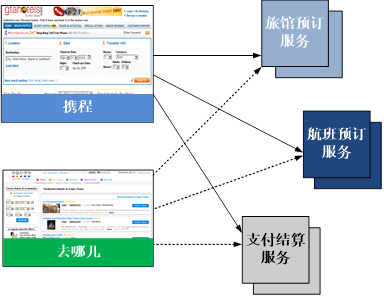
\includegraphics[scale=1]{fig/introduction/cloud_application_instance.png}
			\caption{云应用实例}
			\label{fig_cloud_application_instance}
			\centering\zihao{5}{Fig 1.1 Cloud application instance}
		\end{figure}

		云服务是以互联网为媒介面向用户按需提供的任何一种服务,它的表现形式多样但它的主要特点是能够动态满足用户提交的需求。云服务这一按需提供服务动态特性背后的基础是面向服务架构技术(service-oriented architecture,简写为SOA)。SOA技术在日益竞争激烈的市场环境中扮演着重要的角色,云服务提供商也是采取积极主动的态度大量采用该技术优化自身业务在云环境中的性能。举例来说图\ref{fig_cloud_application_instance}是两个云应用实例,集成了多个云服务包含了旅馆预订,航班预订以及支付结算服务。当用户面对如此功能相似几近相同的云服务,如何区分出这些云服务是用户当前面对的问题,也是学术界的热点。

		图 \ref{fig_The_cloud_architecture}是云服务市场架构示意图。在云环境中,云服务提供商掌握着大量的分布式资源像数据库,这类提供给开发人员设计云服务的资源和平台。当云应用务开发人员需要将多个云服务集成至云应用中,他们需要从云服务市场可用的云服务进行选择。同时这些云服务通常也都是动态地被来自全球各地且由不同通路连接调用进而集成至云应用中。调用云服务的用户往往都是处于不同的地理环境和网络环境。所以当他们在调用这些云服务的时候,连结至云服务的链路都是不同的,这也直接导致用户感受到的云服务质量是不同的。
		\begin{figure}[htb]
			\centering
			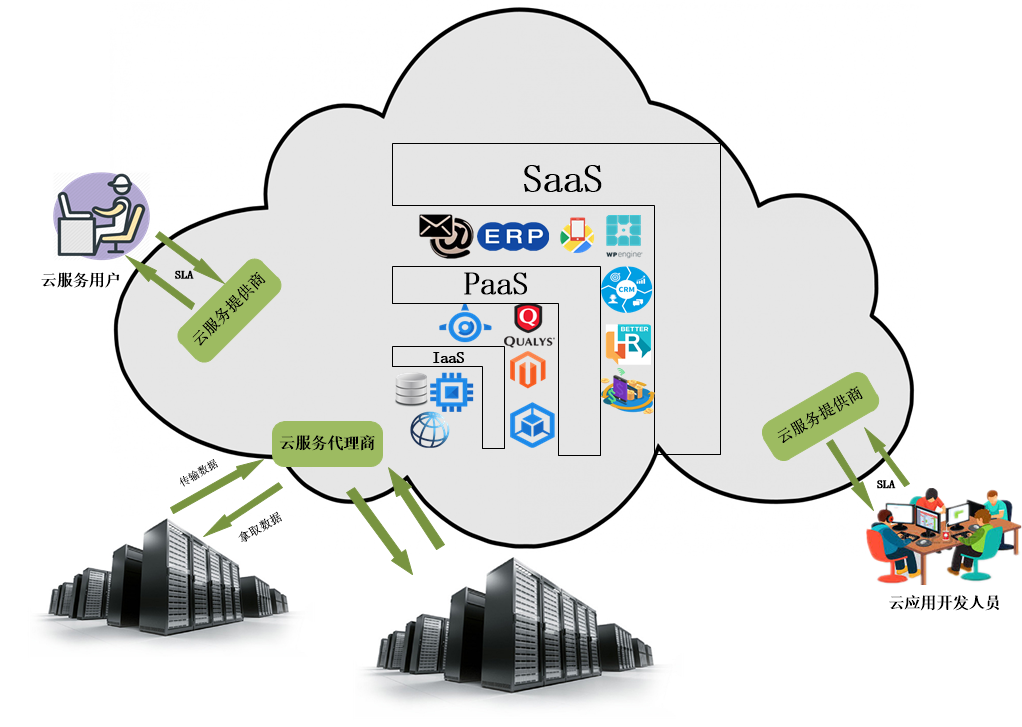
\includegraphics[scale=0.5]{fig/introduction/The_cloud_architecture.png}
			\caption{云市场结构}
			\label{fig_The_cloud_architecture}
			\centering\zihao{5}{Fig 1.2 The cloud architecture}
		\end{figure}
		
		服务质量(Quality of Service,简写为QoS)通常是用来刻画服务的非功能性特点。这也是云应用开发人员在进行云服务选择时十分关心的一个问题。进一步来说,将一些表现得低质的服务替换掉,用一些较好质量的服务取而代之能够整体提高云应用的表现和用户体验。     
		\subsection{研究意义}
		\label{subsec_meaning}
	\section{国内外研究现状}
	\label{sec_current_situation}
	\section{课题研究难点}
	\label{sec_main_points}
	\section{论文主要研究工作}
	\label{sec_main_works}
	\section{论文框架结构}
	\label{sec_paper_architecture}
	%这里是引言\upcite{MATSUMURA2017566,BHATTACHARYYA2010538}。